\chapter{Over-current protection}\label{sec:switch}
The complete over-current protection circuit design can be seen in Figure \ref{fig:circuit_diagram_switch}. Over-current protection was achieved by using an opto-triac circuit to isolate the load from the source voltage once a certain condition was met. An opto-triac is a type of optocoupler circuit that consists of an light emitting device and a light sensing device, which allows a relatively small signal to control a electrically isolated high voltage segment of a circuit \cite{OptoCouplers}. An advantage of using a triac is that it is bidirectional, and can thus allow the flow of current in both halfcycles of the AC supply.\vspace{4mm} \newline  The switching signal for the opto-triac was implemented by using a SR latch that would output a logical high once the trip condition was met. An SR latch is an event driven bistable sequential circuit with two inputs, namely set and reset, where set causes the output to go high, and reset causing the output to go low. The state diagram of the operation of a basic SR latch can be seen in Figure \ref{fig:state_diagram_switch}, showing the relationship between the inputs to the SR latch and the effect of the previous output. The set condition was triggered once a current of more than $\SI{200}{\milli A}$ was detected by the current transducer, this functionality was implemented by using a comparator with its input set as the output from the current transducer, and the reference set as the voltage level equivalent to a current measurement of $\SI{200}{\milli A}$. Once this overcurrent condition was triggered the opto-triac would switch off and remove the supply voltage from the load until the reset condition was set high by the user via a GUI. To protect against over-voltage during the switching process a transient voltage suppression diode was added in parallel with the load.
\begin{figure}[!ht]
  \centering
 \footnotesize
        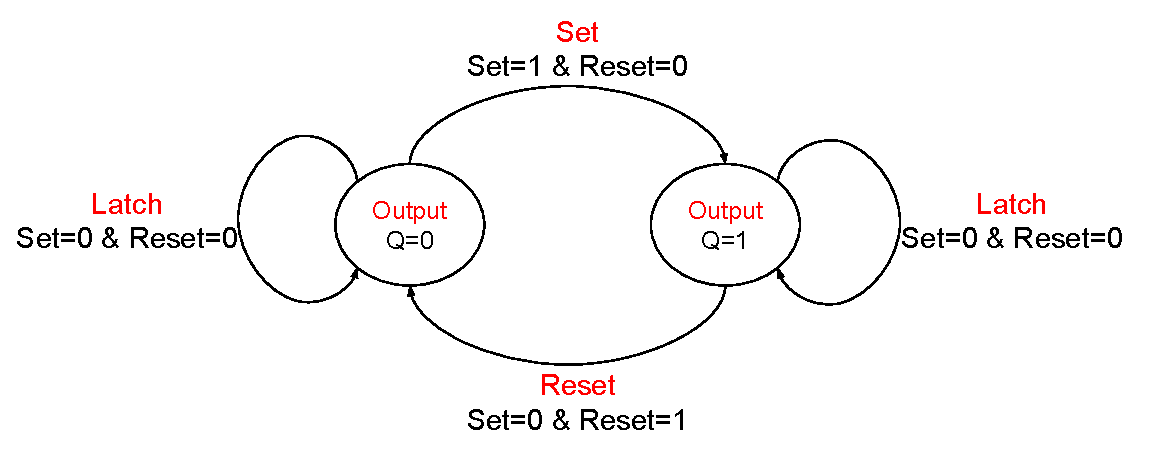
\includegraphics[width=0.65\linewidth]{./Figures/state_diagram_switch.pdf}
    		    \caption{State diagram of a basic SR Latch.} \label{fig:state_diagram_switch}
 \end{figure}

\begin{figure}[!ht]
  \centering
 \footnotesize
        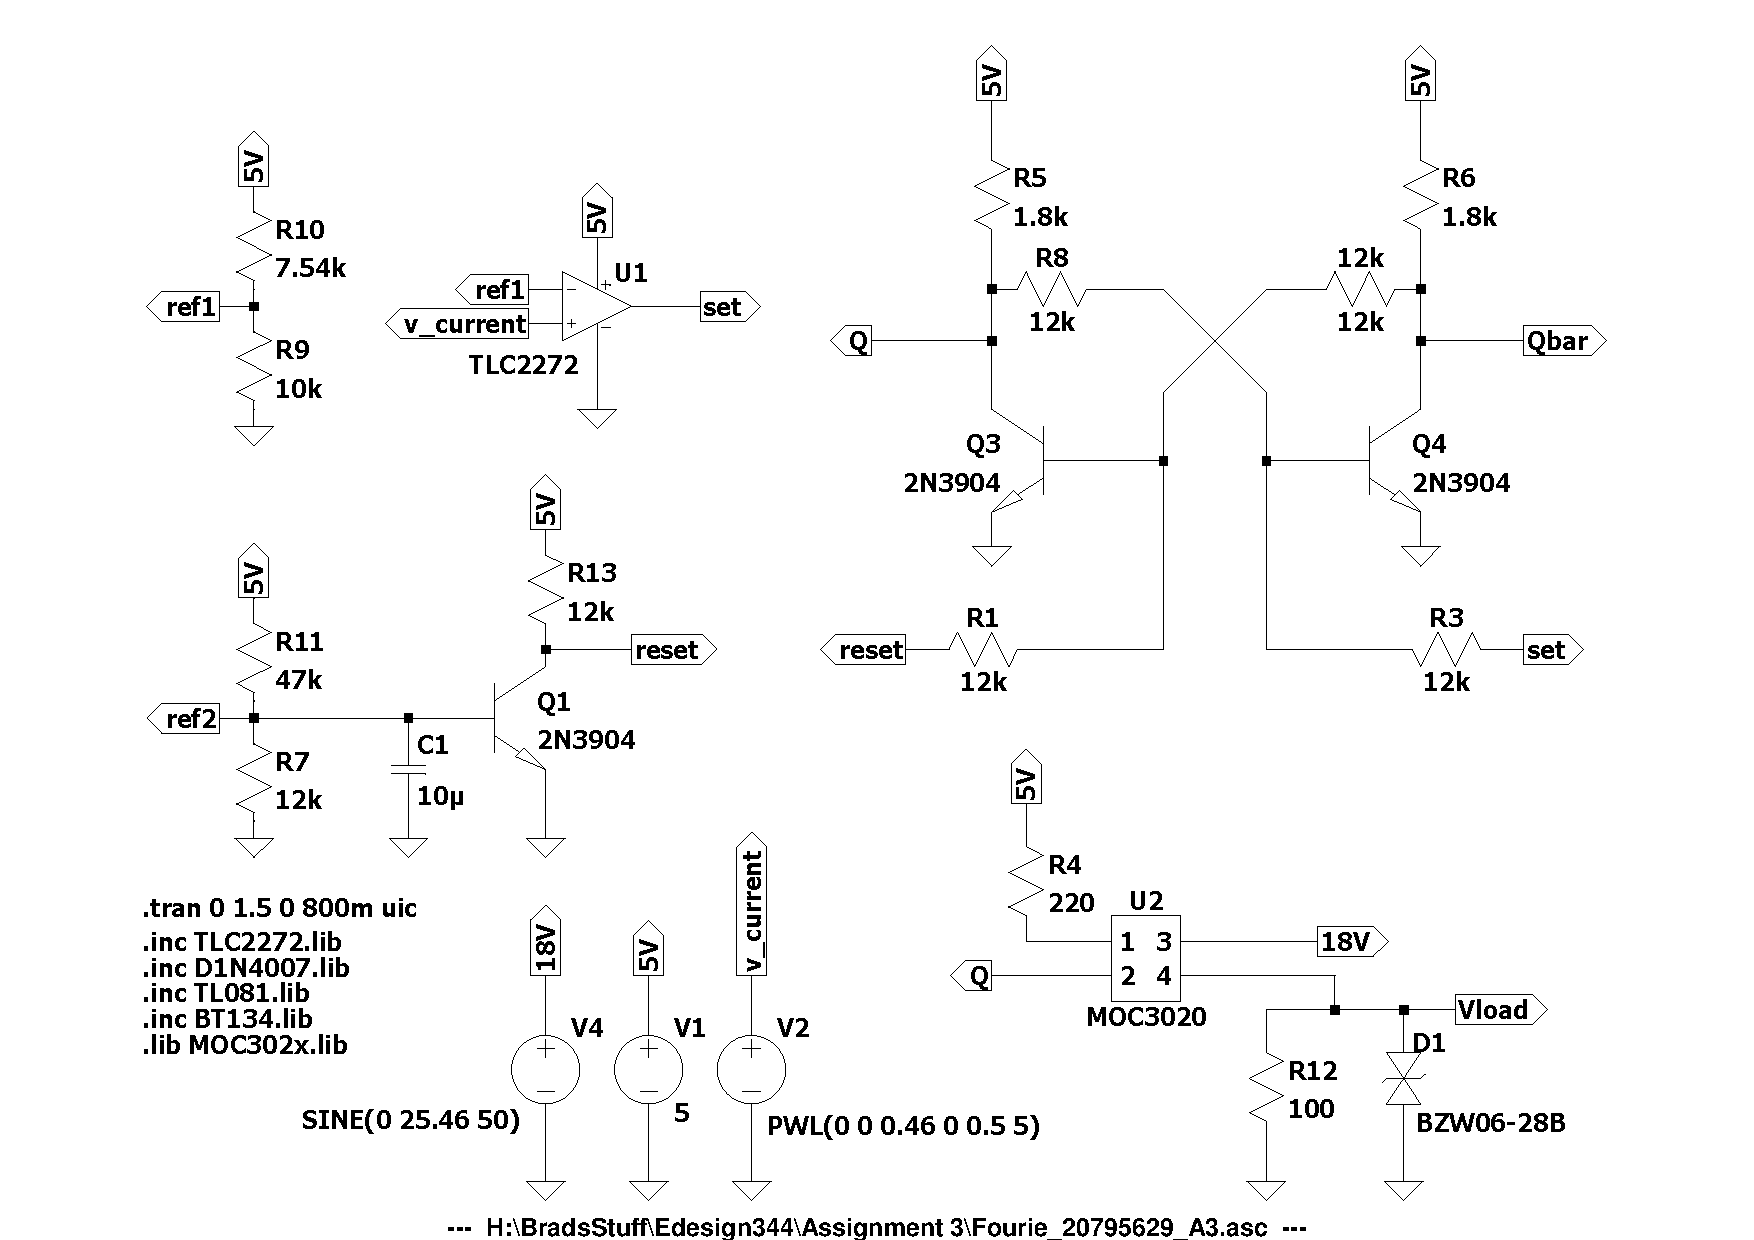
\includegraphics[width=0.75\linewidth]{./Figures/circuit_diagram_switch.pdf}
		    \caption{Over-current protection circuit diagram.} \label{fig:circuit_diagram_switch}
 \end{figure}

\section{Design} \label{sec:sw_design}
The first component of this design that was implemented was the comparator circuitry that would output high when the over-current condition was met. As the input to this comparator was set as the output of the current peak transducer, which could measure currents up to \SI{350}{\milli A}, Equation \ref{eq:currentcalculation} had to be applied to obtain the equivalent voltage level equal to a current draw of \SI{200}{\milli A} chosen as the maximum current allowed through the load. The voltage that would trigger the switch was obtained as $V_{meas}=\frac{I_{load}}{0.0703}=\frac{200m}{0.0703}=\SI{2.85}{V}$, this reference voltage of the comparator was set by using a voltage divider network and choosing a value of $\SI{10}{\kilo \Omega}$ for $R_9$ as to minimise any power losses in the circuit. By Equation \ref{eq:voltagedividerswitch} a value of $\SI{7.54}{\kilo \Omega}$ was obtained for $R_{10}$, and as this was not a standard resistor value a $\SI{10}{\kilo \Omega}$ potentiometer was used and its resistance was changed until the desired reference voltage was obtained.
\begin{align}
   V_{ref}=\frac{R_9}{R_9+R_10}V_{DD}
   \label{eq:voltagedividerswitch}
\end{align}
The SR latch design was realised by using two 2N3904 NPN transistors configured as a bistable multivibrator with two stable states \cite{NPNSRlatch}. To design for the resistor values required all of the possible states of the SR latch had to be taken into consideration. The first consideration that was designed for was the collector current of the transistors, a maximum current would flow through the emitter when the transistor is saturated, with $V_{CE(sat)}=\SI{0.2}{V}$ at the negative terminal of the resistors $R_6$ and $R_5$, and the \SI{5}{V} rail at the positive terminals \cite{2N3904:2003}. In this case the resistors $R_6$ and $R_5$ could be designed for by choosing a maximum collector current of $\SI{2.8}{\milli A}$, the resistors were thus found as $R_6=R_5=\frac{5-0.2}{2.8m}\approx \SI{1.8}{\kilo \Omega}$. \vspace{4mm} \newline To simplify the design calculations resistor values of $\SI{12}{\kilo \Omega}$ was chosen for $R_1$, $R_3$, $R_8$ and $R_{12}$. With these resistor chosen and by setting the value for set high and assuming that the operational amplifier comparator is ideal and has an infinite output resistance, no current will flow through resistor $R_5$, the transistor $Q_3$ would be off and the output of the SR latch would thus be high. On the other side of the SR latch, assuming that reset is low, the base of $Q_4$ would be at $5V$, and thus the transistor would switch on as $V_{BE}>V_{BE(on)}=\SI{0.65}{V}$, and assuming that the transistor saturates the collector of it would at $\SI{0.2}{V}$, which is a logical low \cite{2N3904:2003}. With the output of $Q_4$ at $\SI{0.2}{V}$ and by doing voltage division between $R_1$ and $R_{12}$ we find that the base voltage of transistor $Q_3$ is far below $V_{BE(on)}=\SI{0.65}{V}$, further confirming that the collector of the transistor $Q_3$ is high. The exact reverse is true for the situation where reset goes high and set is low, and for both of these scenarios almost no current will flow through resistors $R_1$, $R_3$, $R_8$ and $R_{12}$, and thus power loss through these resistors is not a problem. Power dissipation in the transistors was found to be at a maximum when each of the transistors saturated, here $P_{Q}=V_{CE(sat)}I_{on}=(0.2)(2.8m)=\SI{0.56}{\milli W}$, which was far below the maximum power dissipation of the 2N3904 \cite{2N3904:2003}. The maximum power dissipation in the resistors used for the SR latch was found with resistors $R_5$ and $R_6$ in the case where $\SI{2.8}{\milli A}$ flowed through them, here $P_{R}=I_{on}^2R=(2.8m)^2(1.8k)=\SI{14.112}{\milli W}$, which was far below the power rating of the $\frac{1}{4}$ Watt resistors used in the design.
\vspace{4mm} \newline 
Finally the opto-triac switch that controlled the load was designed according to the datasheet, where the required forward current of the internal photo-diode required roughly $\SI{24}{\milli A}$ to allow the internal triac to conduct \cite{MOC3020:2000}. The resistor required to allow this current to flow was calculated by considering the situation where $Q_3$ saturates and a collector voltage of $\SI{0.2}{V}$ is present, here $R=\frac{5-0.2}{24m}=200\Omega$. Due to this current flowing into the collector of $Q_3$, in the case where the load is connected to the supply voltage, the power dissipation in the transistor had be recalculated, here $P_{Q(new)}=V_{CE(sat)}I_{on}=(0.2)(2.8m+24m)=\SI{5.36}{\milli W}$, which was as before much less than the maximum power dissipation. It is worth noting that due to the nature of this design no external current gain stage had to be added to the input of the opto-triac.\vspace{4mm} \newline 
A TVS diode was added in parallel with the load as to protect against transient voltage spikes during the switching of the over-current protection circuitry, here a BZW06-28B diode was chosen as it had a reverse breakdown voltage of $\SI{28}{V}$, which was roughly $\SI{3}{V}$ higher than the peak of the nominal supply voltage \cite{BZW06:2016}.\vspace{4mm} \newline
Due to the nature of the SR latch having an undefined output on startup an additional circuit was built as to define the state on startup conditions where the Arduino is disconnected from the computer, refer to Section \ref{sec:extra_func} for more on this.

\section{Simulation} \label{sec:sw_simu}
The over-current functionality for the switch circuitry was tested in simulation by setting reset low, allowing a current to pass through the load and then at a certain time instance to trigger the over-current comparator to output high, the result of this can be seen in Figure \ref{subfig:switch_simu_trip}. From this we can see that the switching circuitry implemented in this design reacted to the over-current condition within 8ms, which was much faster than the 150ms response time required.

\section{Measurements} \label{sec:sw_meas}
The over-current functionality for the switch circuitry was tested with a nominal supply voltage of 18V supplied to a $\SI{1}{\kilo \Omega}$ load. A $\SI{100}{\Omega}$ load was added in parallel to the original load and the trip switch signal as well the response time of the opto-triac was measured on the oscilloscope as shown in Figure \ref{subfig:switch_meas_trip}. From this we can see that the switching circuitry implemented in this design reacted to the over-current condition within 3ms, which was much faster than the 150ms response time required.

\begin{figure}[!ht]
 \footnotesize
 \centering
    \begin{subfigure}[]{0.4\textwidth}
              \centering
  		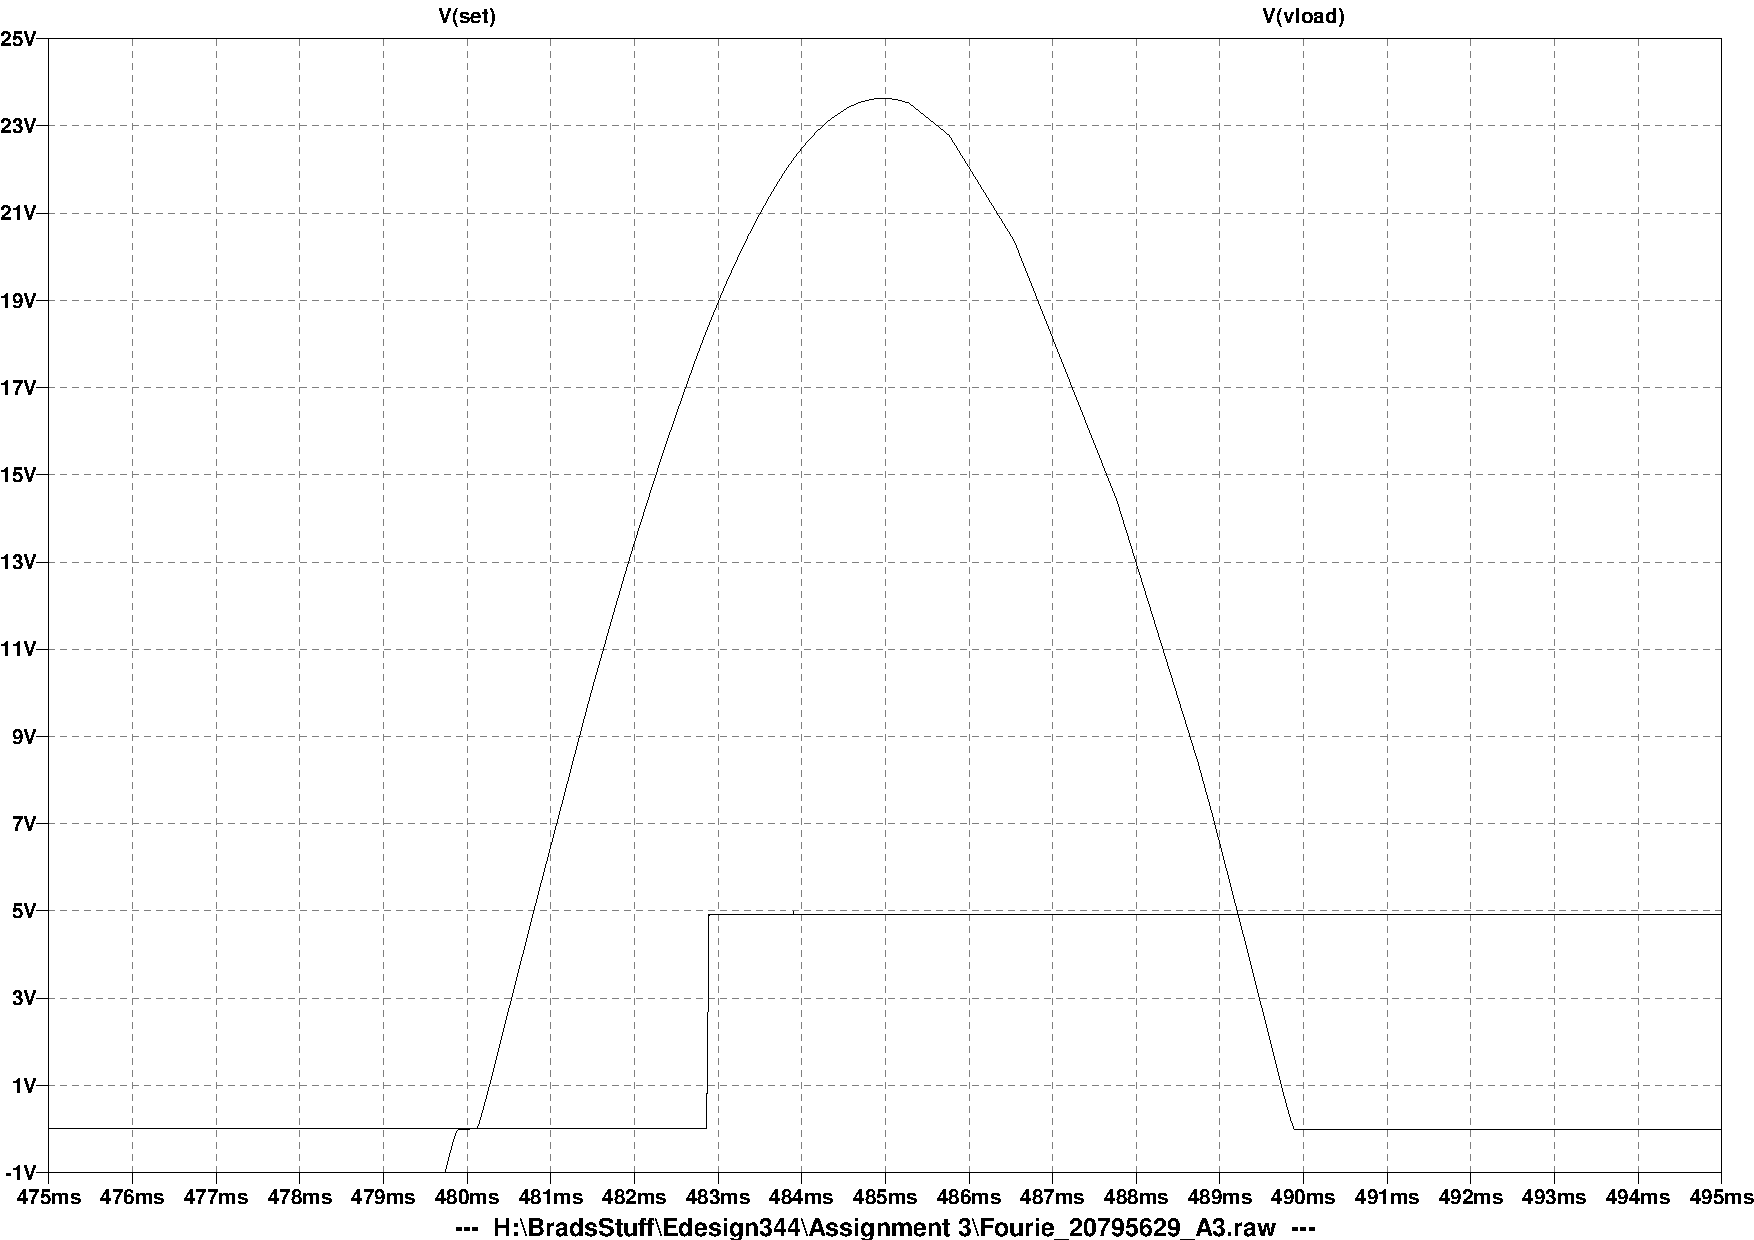
\includegraphics[width=1.0\linewidth]{./Figures/switch_simu_trip.pdf}
		    \caption{} \label{subfig:switch_simu_trip}
     \end{subfigure}
          \begin{subfigure}[]{0.4\textwidth}
             \centering
  		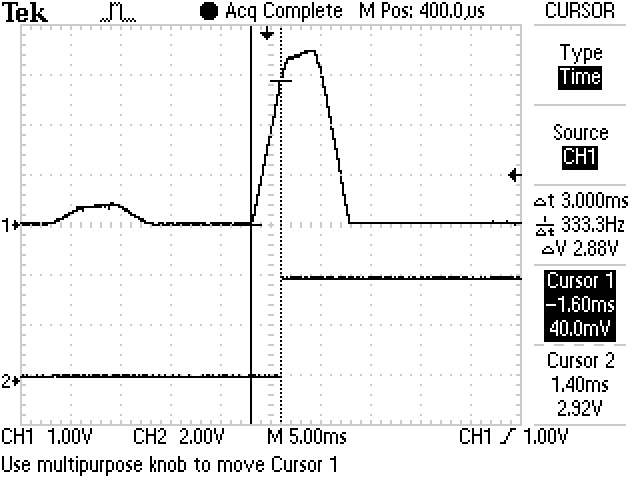
\includegraphics[width=1.0\linewidth]{./Figures/switch_meas_trip.JPG}
		   \caption{ } \label{subfig:switch_meas_trip}
     \end{subfigure}
     \caption[Over-current protection switch results.]{Over-current protection switch results. (a) Set signal and output signal response simulated. (b) Set signal and output signal response measured.} \label{fig:switch_results}
\end{figure}

\section{Summary and implementation}
The switch circuitry was successfully implemented in this design and provided load over-current and surge voltage protection which met all design requirements. The switch circuitry could react to an over-current condition within 3ms and due to the nature of the design the amount of load current that would trigger this overcurrent condition could easily be changed by tuning a potentiometer.

\begin{figure}[h]
    \centering
  		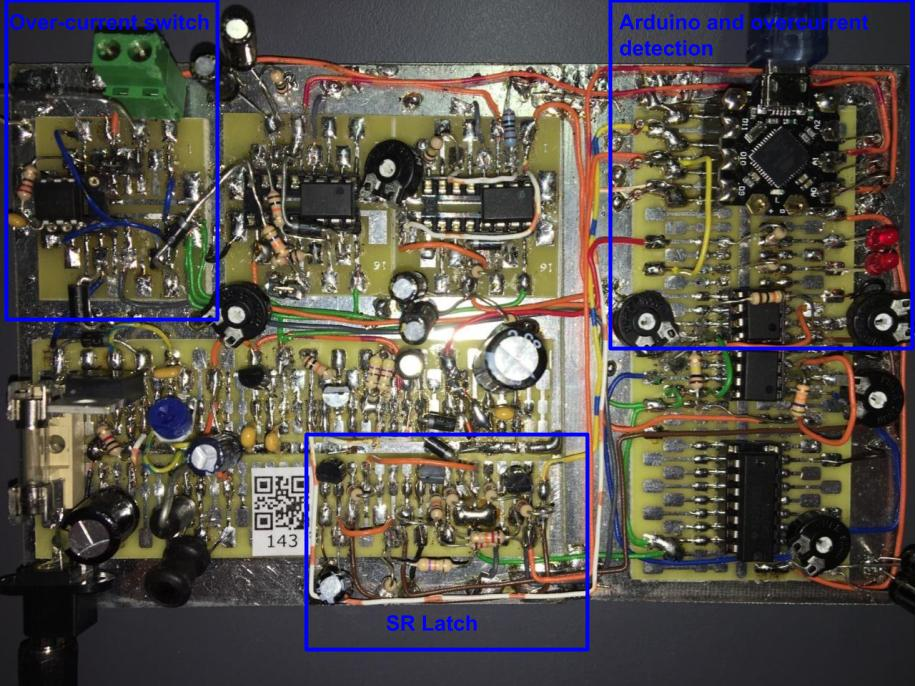
\includegraphics[width=0.45\linewidth]{./Figures/switch_pcb.jpg}
		   \caption{Implementation of the switch circuitry. } \label{subfig:switch_pcb}
     \end{figure}




